\documentclass{beamer}
\usepackage[utf8]{inputenc}
\usepackage[spanish]{babel}
\usepackage{graphics}
\usepackage{graphicx}
\usetheme[secheader=true]{Madrid}
\useinnertheme{rectangles}
\usepackage{tikz}
\title{Memorias}
\subtitle{Velocidad y Volumen}
\author[msagre]{Miguel A Sagreras}
\date[2015]{}
%\institution[short name]{long name}
\begin{document}

\begin{frame}
\titlepage
\end{frame}

\section{Primeras computadoras}
\subsection{Electromecánicas Analógicas}
\begin{frame}
\frametitle{Torpedo Data Computer}
\begin{center}
\hfill
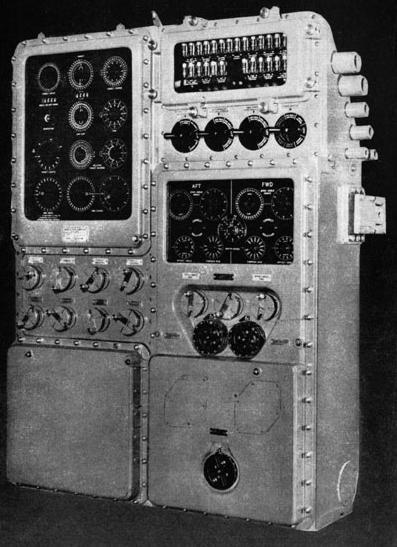
\includegraphics[height=3cm]{TDC-image.jpg}
\hfill
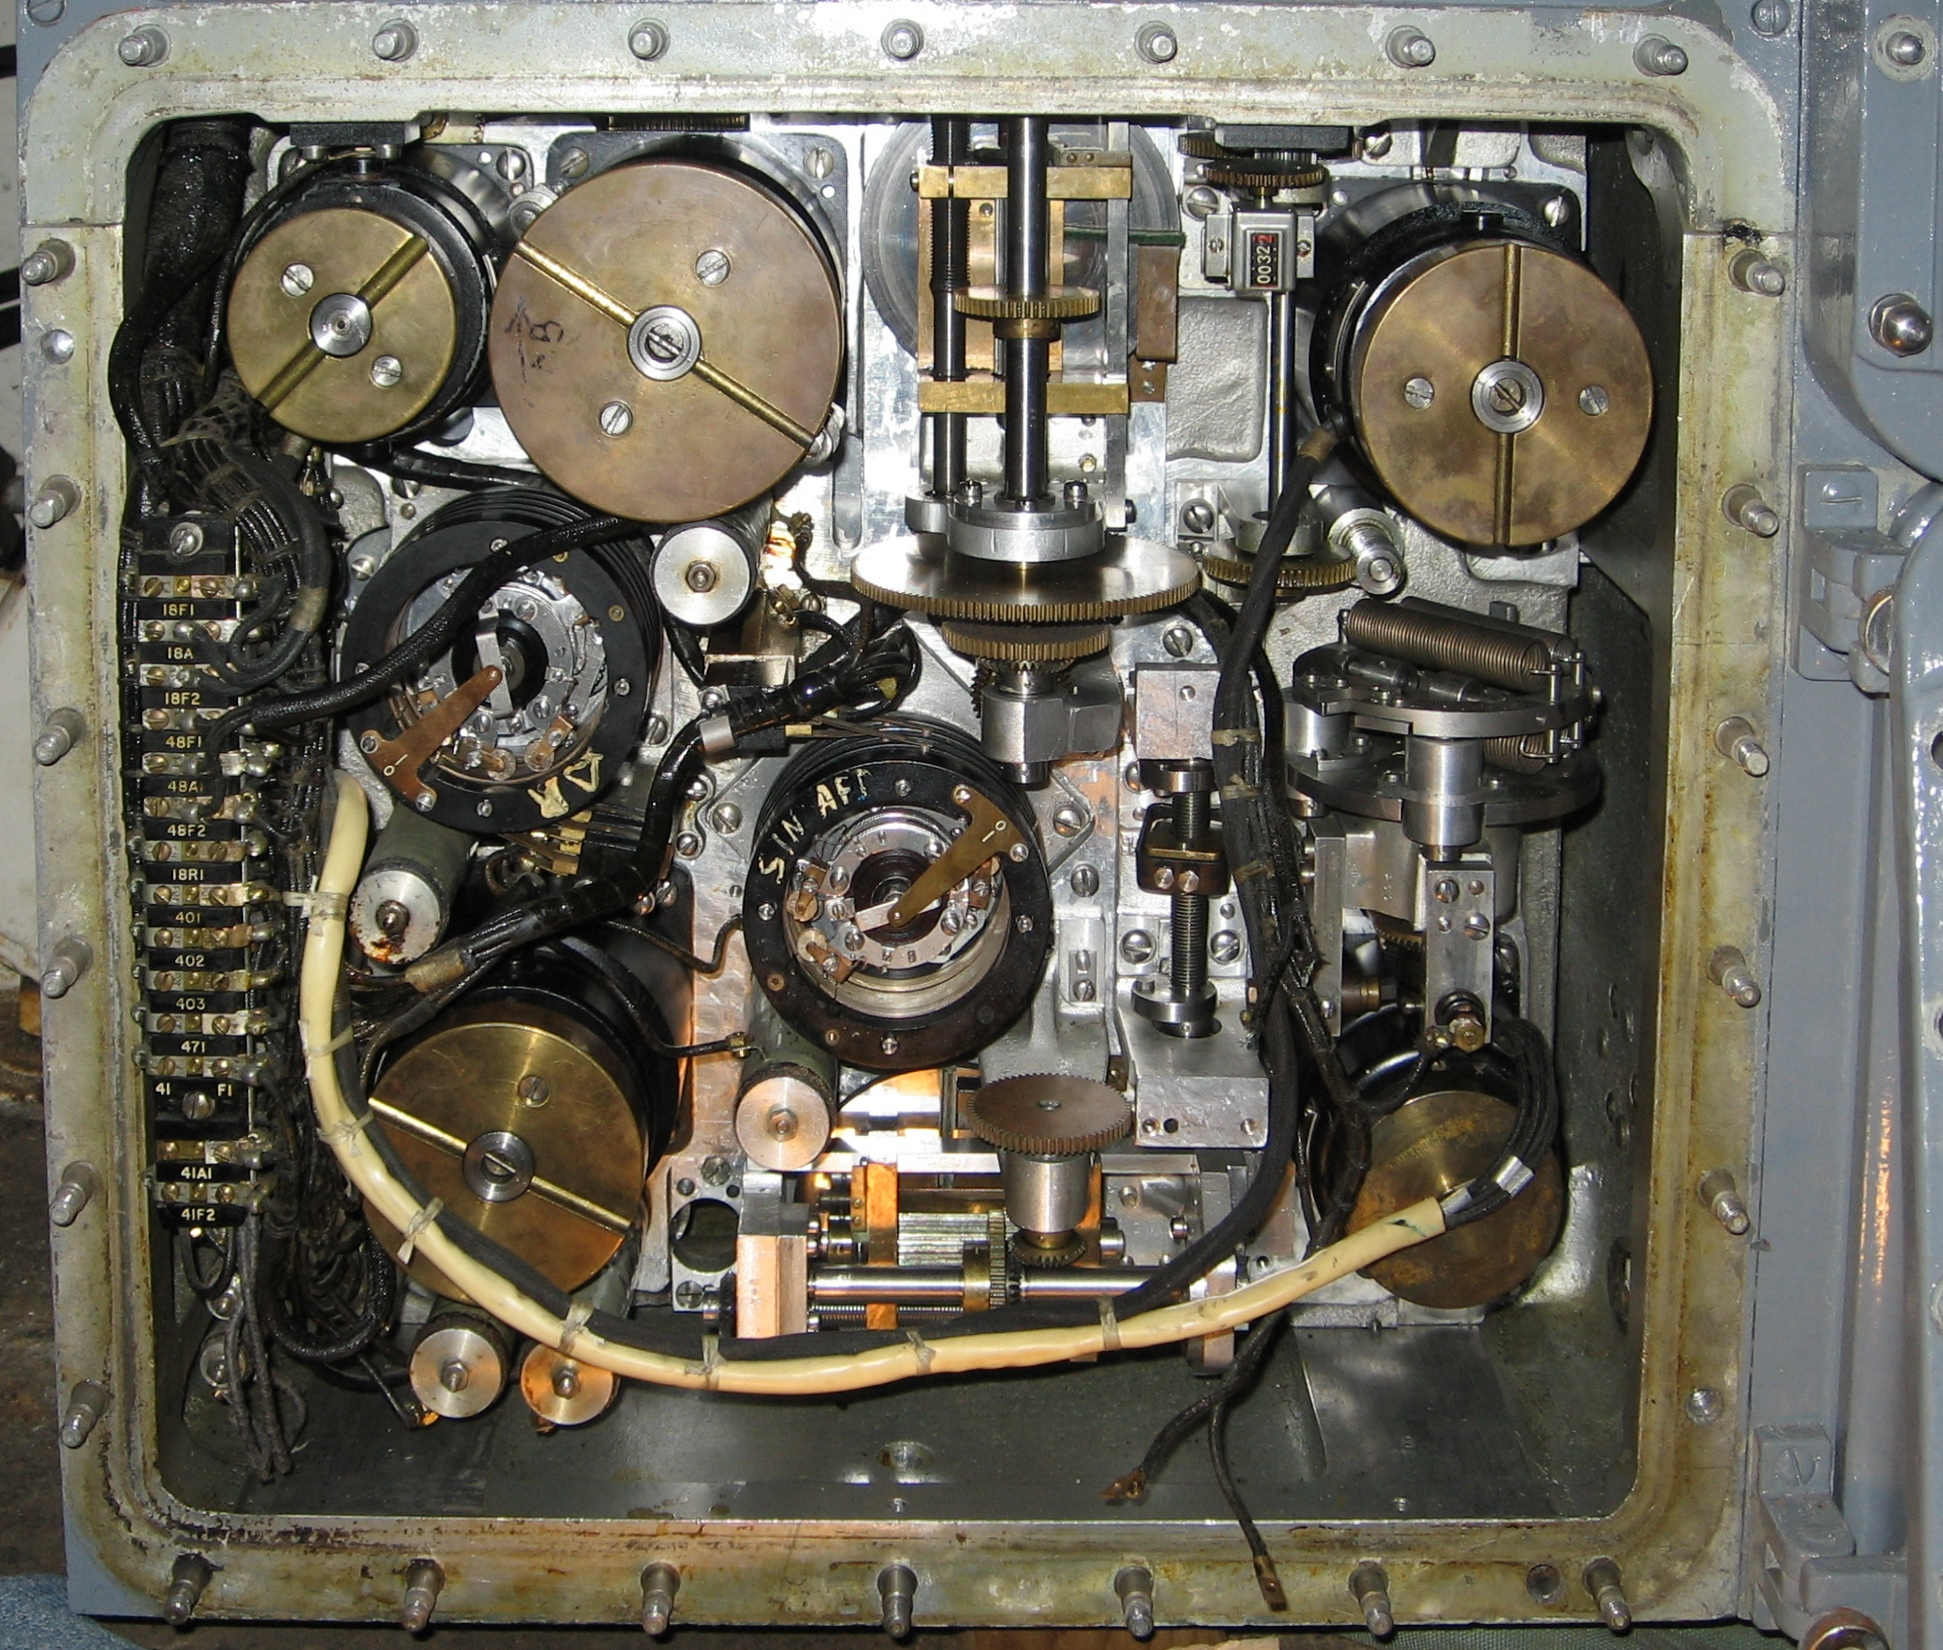
\includegraphics[height=3cm]{TDC-inside.jpg}
\end{center}
\end{frame}

\subsection{Electromecánicas Digitales}
\begin{frame}
\frametitle{Z3}
\begin{itemize}
	\item Año 1941
	\item Diseño Konrad Zuse
	\item Proposito : aeroelasticidad
	\item 2000 relays
	\item Palabra de 22 bits
	\item Memoria 64 palabras
	\item Frecuencia entre 5.3 Hz
	\item 4Kw
	\item 1 Tonelada
\end{itemize}
\begin{center}
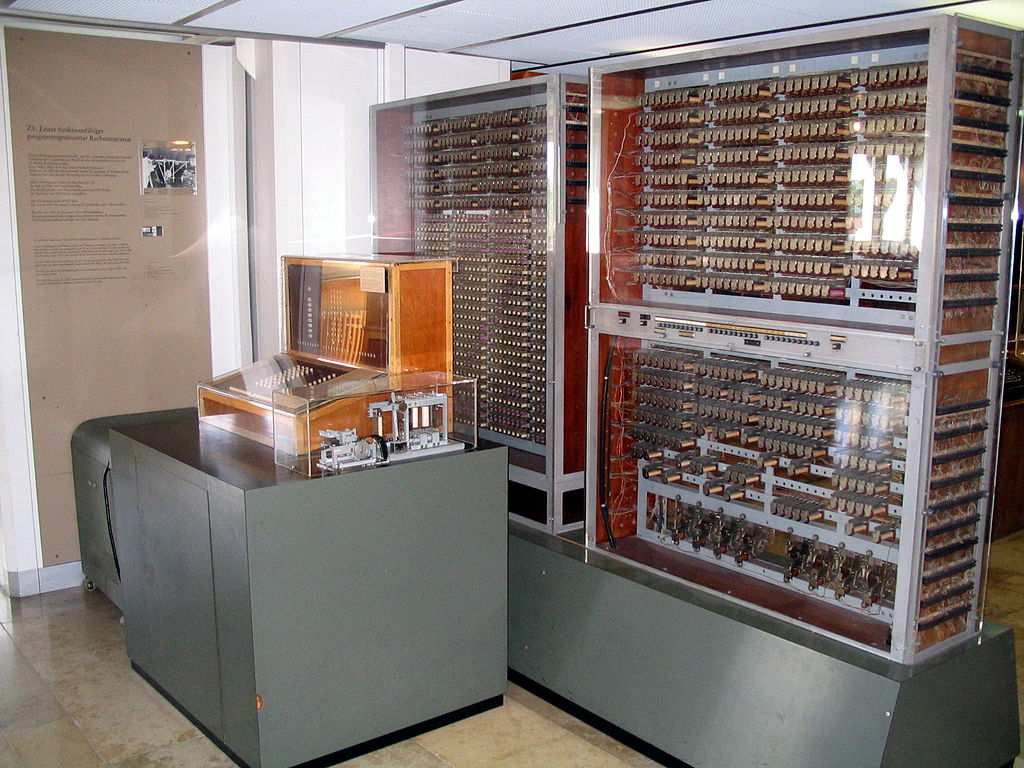
\includegraphics[height=3cm]{Z3_Deutsches_Museum.JPG}
\end{center}
\end{frame}

\subsection{Electromecánicas Digitales}
\begin{frame}
\frametitle{Relays}
\begin{center}
\hfill
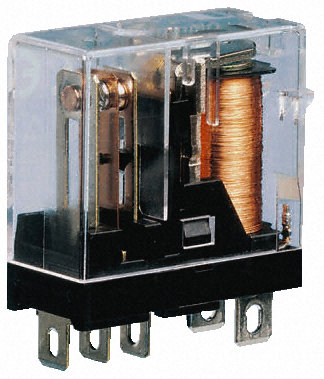
\includegraphics[height=3cm]{relay-imagen.jpg}
\hfill
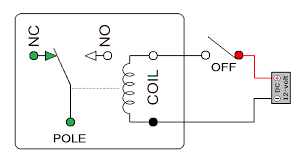
\includegraphics[height=3cm]{relay-diagrama.png}
\end{center}
\end{frame}

\subsection{Electrónicas Digitales}
\begin{frame}
\frametitle{Atanasoff-Berry Computer}
\begin{itemize}
	\item Año 1942
	\item Primera computadora electrócnica 
	\item Resolucion de equaciones diferenciales
	\item mas de 300 tubos de vacio, 320 kg
	\item renerative capacitor memory DRAM 1600 bits
	\item 30 operaciones por segundo, clock the 60 Hz
\end{itemize}
\end{frame}

\begin{frame}
\frametitle{Colssus}
\begin{itemize}
	\item Año 1943-1945
	\item Criptoanalisis
	\item Programación mediante teclas y enchufes
	\item mas de 1600 tubos de vacio
	\item Apodada Colosus por su tamaño.
\end{itemize}
\end{frame}

\begin{frame}
\frametitle{ENIAC}
\begin{itemize}
	\item Año 1943
	\item Cálculo de trayectoria de misiles
	\item Programación mediante teclas y enchufes
	\item Recursos
		\begin{itemize}
			\item más de 17000 tubos de vacio
			\item 7.200 diodos de cristal
			\item 70.000 resistencias
			\item 10.000 capacitores
			\item 5.000.000 de soldaduras
			\item 150Kw
			\item 167 mm2
			\item 500.000 de dollares
			\item Memoria 100 palabras de 10 digitos decimales o 1000 bytes
		\end{itemize}
\end{itemize}
\end{frame}

\begin{frame}
\frametitle{EDSAC}
\begin{itemize}
	\item Año 1949
	\item Cálculo de trayectoria de misiles
	\item Programación mediante teclas y enchufes
	\item Recursos
		\begin{itemize}
			\item Tubos de vacio como logica
			\item Memoria Lineas de Retardo de mercurio
			\item Capacidad 1024 palabras de 36 bits en 1955
		\end{itemize}
\end{itemize}
\end{frame}

\subsection{Memoria}
\begin{frame}
\frametitle{Memoria de linea de retardo}
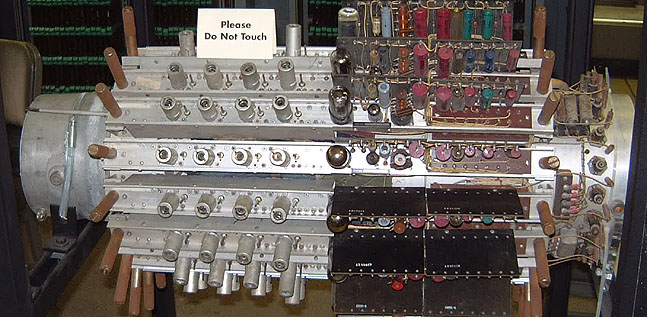
\includegraphics[height=3cm]{Mercury_memory.jpg}
\end{frame}

\subsection{Memoria}
\begin{frame}
\frametitle{Memoria de linea de retardo}
\begin{itemize}
	\item John Adam Presper Eckert
	\item Origen en las lineas de retardo para Radar
	\item Medio de propagación Mercurio
		\begin{itemize}
			\item Rápida velocidad de propagación del sonido 1450m/s
			\item Impendancia acoustica similar a la del crystal 
		\end{itemize}
\end{itemize}
\end{frame}

\begin{frame}
\frametitle{Drum memory}
\begin{itemize}
	\item Gustav Tauschek
\end{itemize}
\end{frame}

\subsection{Memoria}
\begin{frame}
\frametitle{Memoria de linea de retardo}
\begin{itemize}
	\item John Adam Presper Eckert
	\item Origen en las lineas de retardo para Radar
	\item Medio de propagación Mercurio
		\begin{itemize}
			\item Rápida velocidad de propagación del sonido 1450m/s
			\item Impendancia acoustica similar a la del crystal 
		\end{itemize}
\end{itemize}
\end{frame}

\section{Memoria}
\begin{frame}
\frametitle{Estructura de la  memoria dinámica}
\begin{figure}[!htb]
\centering
\includegraphics[scale=0.8]{membank.eps}
\end{figure}
\end{frame}

\section{Banco de Memoria}
\begin{frame}
\begin{figure}[!htb]
\centering
\includegraphics[scale=1.0]{chip.eps}
\end{figure}
\end{frame}

\section{Secuencia de acceso}
\begin{frame}
	\begin{itemize}
		\item Acceder a la fila
		\item Acceder a la columna
		\item Recuperar el valor leido
	\end{itemize}
\end{frame}

\section{Timing diagram}
\begin{frame}
\begin{figure}[!htb]
\centering
\includegraphics[scale=1.0]{dram-timings.eps}
\end{figure}
\end{frame}

\section{Timing diagram}
\begin{frame}
\begin{figure}[!htb]
\centering
\includegraphics[scale=1.0]{ddrdram-timings.eps}
\end{figure}
\end{frame}

\section{fpga}
\begin{frame}
\begin{figure}[!htb]
\centering
\includegraphics[scale=1.0]{fpga.eps}
\end{figure}
\end{frame}

\end{document}

